\documentclass[a4paper,12pt]{article}

% 导言区
\usepackage{titlesec}
\usepackage{lipsum} % 示例用,可以删除
\usepackage{geometry}
\usepackage{setspace}
\usepackage{amsmath} % 用于数学公式
\usepackage{graphicx} % 用于插入图片
\usepackage{lipsum} % 用于生成虚拟文本
\usepackage{ctex} % 导入 ctex 包以支持中文
\usepackage{titlesec} % 导入 titlesec 包以定制标题样式
\usepackage{fontspec} % 用于设置中文字体
\usepackage{amsfonts} 
\usepackage{amsmath} % 提供 \text 和 \tanh 命令
\usepackage{bm}      % 提供 \bm 命令用于粗体
% 目录设置
\usepackage[nottoc,notlot,notlof]{tocbibind}
\usepackage{enumitem}
% 页面设置
\geometry{margin=1in}

% 标题设置
\titleformat{\section}{\normalfont\Large\bfseries}{\thesection}{1em}{}
\titleformat{\subsection}{\normalfont\large\bfseries}{\thesubsection}{1em}{}
\titleformat{\subsubsection}{\normalfont\normalsize\bfseries}{\thesubsubsection}{1em}{}

% 行间距设置
\onehalfspacing

% 文档信息
\title{项目启动文档}
\author{软件学院:程智镝,刘辉,陈凌,李忠信}
\date{\today}

\begin{document}

\maketitle

% 添加目录
\tableofcontents

\section{项目概要}

\subsection{项目选题}
一款面向大众的虚拟会议软件,名称TODO
\subsection{团队成员}
程智镝,211250124
刘辉,211250122
陈凌,211250159
李忠信,211250158
\subsection{度量数值}
本文档共包含TODO个要点与TODO个关联关系,平均要点数量为TODO个。

要点之间的关联详见第4部分
% 添加目录
\tableofcontents
\section{项目简介}
项目旨在帮助用户在任何地点和任何时间进行高质量的在线会议和协作,从各个维度满足用户对于远程会议的需要。通过提供音频、视频、文字聊天、文件共享和屏幕共享等功能来促进沟通和协作。主要目标是提供一个安全、可靠、用户友好的平台,从小型团队会议到大型企业级活动满足各种用户需求。

项目的根本出发点是基本会议功能。支持用户创建和加入会议,支持同时多人在线会议。允许用户共享他的屏幕,方便在会议中展示演示文稿,应用程序或是其他内容。支持文字聊天,提供实时文本聊天服务,方便在会议期间交流和提问。允许用户单向屏蔽,选择性的不接收来自某人的消息以及音视频聊天。支持会议禁言成员。允许用户设置自动保存会议回放至本地及云端。

我们新增了日历集成功能,与日历应用程序合作,方便用户安排会议时间并向会议成员发送提醒。添加了会议规划的功能,用户可以查看会议的历史记录,以及将未来的会议添加到会议规划,也就是日历中,在会议开始前会向用户发送提醒,避免遗忘而错过会议。
为了不错过每次会议的精彩瞬间,我们添加了可以自行选择开关的会议自动备份功能,会议持有者选择开启后,会议成员在申请通过后可以在云端查看此次会议的回放并提供下载到本地的服务。我们提供了文件共享和云存储集成功能,一方面,允许用户在实时会议中发送文件,图片以及文档,方便实时交流和讨论;另一方面,与云存储服务如OneDrive,DropBox集成,便于存储文件和重复查看。

我们引入了社交系统,对已存在联系人列表中的其他用户,用户可以直接在应用中发出会议邀请,好友会收到入会邀请。我们同时开放了广场功能,即开放的会议室,让会议不只局限于严肃的教学和组会中,尝试将会议功能娱乐化,用户可以在本地或者添加网址链接的方式选择一段音乐或是电影,邀请好友共同观看,或是创建一个公开房间,允许大厅中的陌生人加入你一同听歌或是观影,并可以通过语音,文字实时交流,通过添加好友的功能去开启一段崭新的邂逅之旅吧!同时,类似于公开课之类的学习课程也可以在广场中面向所有有学习需求的用户开放,通过对主题的筛选,用户可以很方便的找到想要加入的公开会议。让会议不再只是熟人之间的工具,也成为陌生人之间分享与沟通的桥梁。

我们对企业所需求的会议进行了专门的加密隐私处理,提供端到端加密以保护会议内容的隐私安全。通过申请发起企业会议权限,用户可以创建一个更具安全性保密性的会议,首先,加入会议的成员需要通过会议持有者审核才可加入会议,其次,支持多人同时共享,多设备同时操作,让入会者更加高效办公。用户可以与之前提到的日历功能配合使用,预定周期性的会议,不再需要每次提前准备申请企业会议,减少重复操作次数。

我们针对教育需求新增了教学会议功能,提供了面向线上课堂的专属会议模块,添加了诸如小组讨论,举手答题,课堂小测等功能,课堂回放保存至云端可以随时访问,尽可能地模拟线下课堂的环境,结合线上教学的优势条件,让智能教学更加普及。

% 添加目录
\tableofcontents
\section{商业模式画布}
\textbf{画布}
\begin{figure}[htbp]
    \centering
    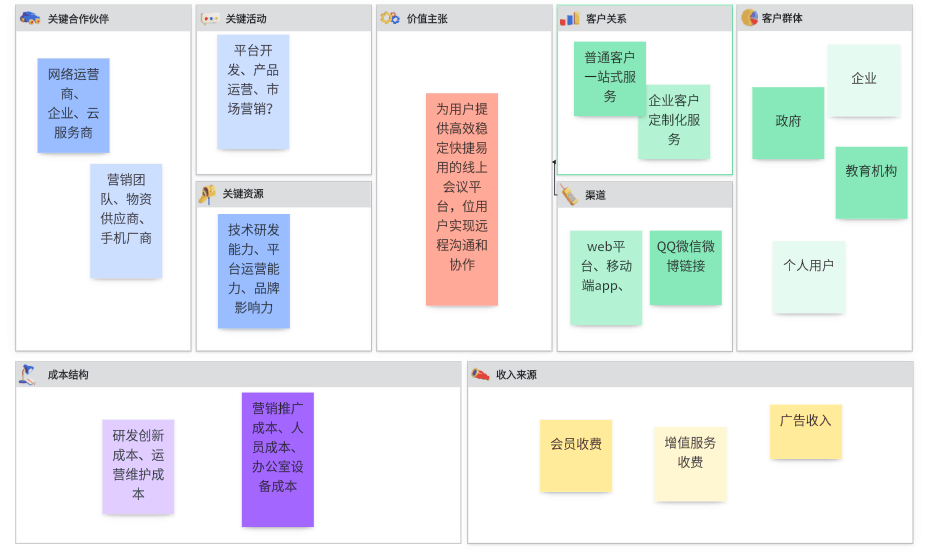
\includegraphics[scale=0.5]{腾讯会议商业模式画布.png}
    \caption{figure title}
    \label{figure}
\end{figure}

\textbf{要点讲解}
\subsection{关键合作伙伴}
\begin{itemize}[label=--, left=0pt]
    \item 网络运营商:腾讯会议需要合作网络运营商确保高质量的网络连接,尤其是在视频会议等需要大带宽的场景。
    \item 企业:合作企业可能提供定制化解决方案、集成服务或其他支持,以满足企业级用户的特殊需求。
    \item 云服务商:与云服务商的合作有助于提高会议平台的弹性、可伸缩性,并提供高效的存储和计算资源。
    \item 营销团队:营销团队的合作将有助于推广和宣传腾讯会议,吸引更多用户,尤其是企业用户。
    \item 物资供应商:物资供应商可能提供与硬件设备、办公室设备等相关的支持和服务。
\end{itemize}

\subsection{关键活动}
\begin{itemize}[label=--, left=0pt]
    \item 平台开发:持续的技术研发和平台开发是确保腾讯会议保持竞争力和创新的关键活动。
    \item 产品运营:有效的产品运营确保用户体验优越,功能得到充分利用,并满足不断变化的用户需求。
    \item 市场营销:强大的市场营销活动有助于提高品牌知名度,吸引新用户,尤其是在竞争激烈的在线会议市场。
\end{itemize}

\subsection{关键资源}
\begin{itemize}[label=--, left=0pt]
    \item 技术研发能力:这是腾讯会议成功的核心,需要持续投资和保持领先的技术水平。
    \item 平台运营能力:有效的平台运营确保服务的可靠性、稳定性和高效性。
    \item 品牌影响力:强大的品牌影响力可以吸引更多用户,建立信任,并为腾讯会议带来竞争优势。
\end{itemize}

\subsection{成本结构}
\begin{itemize}[label=--, left=0pt]
    \item 研发创新成本:高水平的研发投入是必不可少的,以确保平台的不断创新和领先地位。
    \item 运营维护成本:保持平台的稳定性和可用性需要不断的运营和维护工作。
    \item 营销推广成本:在激烈的市场竞争中,有效的营销是必要的,但也需要控制成本。
    \item 人员成本:涵盖研发、运营、营销等方面的人员成本。
    \item 办公室设备成本:包括办公空间、硬件设备等的成本。
\end{itemize}

\subsection{价值主张}
腾讯会议提供高效、稳定、快捷、易用的线上会议平台,为用户实现远程沟通和协作,满足了用户的实际需求。

\subsection{客户关系}
\begin{itemize}[label=--, left=0pt]
    \item 私人服务:为个人用户提供个性化的服务和支持。
    \item 自助服务:提供简便易用的自助服务工具,使用户能够更好地管理其会议体验。
    \item 客户协作:与企业客户建立密切的合作关系,以满足其特定需求。
    \item 社区:建立用户社区,促进用户之间的互动和信息共享。
\end{itemize}

\subsection{渠道}
\begin{itemize}[label=--, left=0pt]
    \item Web平台、移动端App:主要的服务传递渠道,满足用户在不同设备上的需求。
    \item QQ微信微博链接:通过社交媒体渠道进行推广,扩大用户基础。
\end{itemize}

\subsection{收入}
\begin{itemize}[label=--, left=0pt]
    \item 会员收费:提供高级会员服务,收取会员费用。
    \item 增值服务收费:提供一些额外的增值服务,如大规模会议、高级安全功能等,以获取额外收入。
    \item 广告收入:在免费版本中通过广告获取收入。
\end{itemize}

\subsection{客户群体}
\begin{itemize}[label=--, left=0pt]
    \item 企业
    \item 政府
    \item 教育机构
    \item 个人用户
\end{itemize}
% 添加目录
\tableofcontents
\section{要点关联}

% 添加目录
\tableofcontents
\section{问题域}
TODO
\end{document}
